% !TEX program = xelatex

\documentclass[aspectratio=169]{beamer}

\usepackage{xltxtra} 
\usepackage{fontspec}
\usepackage{listings}
\usepackage{color}
\usepackage{amsmath}
\usepackage{smartdiagram}
\usepackage{graphicx}
\usepackage{multicol}
\usepackage{tikz}
\usetheme{metropolis}
\XeTeXlinebreaklocale "th_TH"
\defaultfontfeatures{Mapping=tex-text,Scale=MatchLowercase}

\title{Python for Data Science}
\author{Sirakorn Lamyai}
\institute{Student, Kasetsart U.}

\begin{document}
\maketitle

\begin{frame}
    \frametitle{About me}
    \begin{columns}
        \column{0.3\textwidth}
            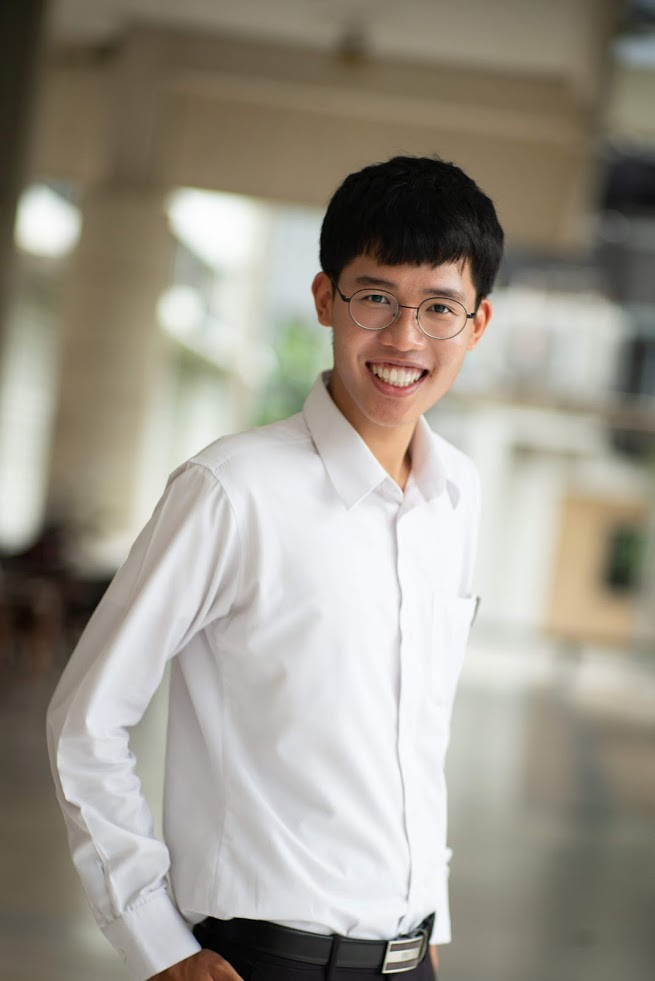
\includegraphics[height=0.8\textheight]{images/sirakorn-1.jpeg}
        \column{0.7\textwidth}
            {\large \textbf{Sirakorn Lamyai}}
            \begin{itemize}
                \item DAKDL Laboratory, Kasetsart University
                \item Research Assistant Intern, 2019, Vidyasirimedhi Institute of Science and Technology
                \item Research Assistant Intern, 2018, Vidyasirimedhi Institute of Science and Technology
                \item Love drinking tea
                \item Knows a little about Python
            \end{itemize}
    \end{columns}
\end{frame}

\begin{frame}
    \frametitle{I know a little about Python}
    When I say I know \textit{a little} about Python\dots
    \begin{itemize}
        \item I think there's some better methods than I'm using
        \item I think I do sometimes make mistakes
        \item There are tons of people who know things much more than me
        \item I think there's much more for me to learn!
    \end{itemize}
\end{frame}

\begin{frame}
    \frametitle{Prerequisite}
    A basic Python knowledge will do!
\end{frame}

\begin{frame}
    \frametitle{Your expectations from this talk}
\end{frame}

\begin{frame}
	\frametitle{Outline}
    \tableofcontents
\end{frame}

\section{Data Science}

\begin{frame}
    \frametitle{The Data Science Process: OSEMNI}
    \begin{itemize}
        \item \textbf{Obtain} data from relevent sources
        \item \textbf{Scrub}, sanitise, and clean the data into machine-understandable formats
        \item \textbf{Explore} significant and meaningful patterns with statistical methods
        \item \textbf{Model} construction for prediction and forecast
        \item \textbf{iNterpret} and use the results obtained
        \item \textbf{Interate} and rethink about your outputs
    \end{itemize}
\end{frame}

\end{document}
